\documentclass[12pt]{article}
%\usepackage{amsmath}
\usepackage{graphicx}
%\usepackage{enumerate}
\usepackage{natbib} %comment out if you do not have the package
\usepackage{url}
 % not crucial - just used below for the URL 
\usepackage{amsmath, amssymb}
\usepackage{setspace} % NOT IN TECHNOMETRICS TEMPLATE
\usepackage{caption} % NOT IN TECHNOMETRICS TEMPLATE



%\pdfminorversion=4
% NOTE: To produce blinded version, replace "0" with "1" below.
\newcommand{\blind}{0}

% DON'T change margins - should be 1 inch all around.
\addtolength{\oddsidemargin}{-.5in}%
\addtolength{\evensidemargin}{-.5in}%
\addtolength{\textwidth}{1in}%
\addtolength{\textheight}{1.3in}%
\addtolength{\topmargin}{-.8in}%

\date{}
\begin{document}

%\bibliographystyle{natbib}

\def\spacingset#1{\renewcommand{\baselinestretch}%
{#1}\small\normalsize} \spacingset{1}


%%%%%%%%%%%%%%%%%%%%%%%%%%%%%%%%%%%%%%%%%%%%%%%%%%%%%%%%%%%%%%%%%%%%%%%%%%%%%%

\if0\blind
{
  \title{\bf Combining model calibration and design}
  \author{Carl Ehrett\thanks{
    The authors gratefully acknowledge \textit{please remember to list all relevant funding sources in the unblinded version}}\hspace{.2cm}\\
    School of Mathematical and Statistical Sciences, Clemson University,\\
    D. Andrew Brown \\
    School of Mathematical and Statistical Sciences, Clemson University,\\
    Evan Chodora \\
    Department of Mechanical Engineering, Clemson University,\\
    Christopher Kitchens \\
    Department of Chemical and Biomolecular Engineering, Clemson University,\\
    and \\
    Sez Atamturktur \\
    Department of Architectural Engineering, Pennsylvania State University\\}
  \maketitle
} \fi

\if1\blind
{
  \bigskip
  \bigskip
  \bigskip
  \begin{center}
    {\LARGE\bf Title}
\end{center}
  \medskip
} \fi

\bigskip
%\begin{abstract}
%Abstract
%\end{abstract}

\noindent%
{\it Keywords:}  
\vfill

\newpage
\spacingset{2} % DON'T change the spacing!
\section{Introduction}
\label{introduction}

%
The goal of traditional Kennedy-O'Hagan style calibration \citep[KOH, ][]{kennedy2001} is to find a posterior distribution on unknown parameters by calibrating a computer model using real-world observations of the modeled phenomenon.
%
By contrast, the design methodology of calibration to target outcomes (CTO) uses the KOH framework to find a posterior distribution on optimal input settings in the model by ``calibrating'' a computer model using artificial observations that reflect performance and cost targets for the modeled system.
%
The goal of the work described here is to combine KOH and CTO.
%
Call the resulting methodology DCTO, for dual calibration to target outcomes.

CTO as previously developed assumes, somewhat idealistically, that the computer model is already perfectly calibrated.
%
DCTO avoids this idealization.
%
Furthermore, when undertaking KOH, some areas of the model range may be of greater interest than others.
%
For example, one may be more interested in calibrating the model to be accurate in the optimal region of some design variable $\theta$ than elsewhere.
%
Undertaking dual calibration may allow us to focus our calibration efforts on such regions of interest, prioritizing them over other areas of the model range.
%

%
\section{Na\"ive DCTO}
%% Describe KOH model
%
The version of KOH considered here is that which finds a posterior distribution on a parameter of interest, $\boldsymbol\theta$, using a GP emulator with hyperparameters $\widehat{\boldsymbol\phi_\eta}$ estimated via maximum likelihood using a budget of computer model observations $\boldsymbol\eta$. 
%
Similarly, we use a GP prior with hyperparameters $\phi_\delta$ to model discrepancy between the computer model $\eta()$ and the true function $f()$ that it represents.
%
In the work described here, we employ stationary GPs with a Gaussian kernel covariance structure $C(\mathbf x,\mathbf x') = 1/\lambda \times \exp(-\beta(\mathbf x-\mathbf x')^2)$, so that $\widehat {\boldsymbol\phi_\eta} = \left[\widehat \beta,\ \widehat \lambda\right]$.
%
Setting priors on $\boldsymbol\theta$ and on $\phi_\delta$, we train the GP emulator on observations $\boldsymbol \eta$ and use MCMC to explore the distribution
\begin{equation} \label{eq:full_dist}
\pi(\boldsymbol \theta,\phi_\delta|\mathcal D,\widehat{\phi_\eta})
\propto \pi(\mathcal D | \boldsymbol \theta,\widehat{\phi_\eta}, \phi_\delta) %\times \pi(\lambda_\eta) 
%\times \pi(\boldsymbol \rho^\eta) 
\times \pi(\boldsymbol\theta)
\times \pi(\phi_\delta)
\end{equation}
%
where $\mathcal D = (\boldsymbol\eta^T,\ \mathbf y^T)^T$.
%

%
In a computer calibration problem, $\mathbf y$ is a set of observations of the system modeled by $\eta()$.
%
In CTO, by contrast, $y$ is a set of target outcomes -- artificial data representing the way that one wishes to induce the system to behave, rather than observations one has made of the system in reality.
%
When one wishes to perform CTO on a system that also requires traditional calibration, then, one obvious idea is to combine the two approaches by using Equation \eqref{eq:full_dist} with $\mathbf y= (\mathbf y_r^T,\ \mathbf y_t^T)^T$, an array containing both real observations $\mathbf y_r$ (for calibration) and target outcomes $\mathbf y_t$ (for CTO).
%
However, this approach will not work, for two reasons.
%
Firstly, the inputs $\boldsymbol\theta$ are typically not the same in calibration and in CTO.
%
In calibration, one seeks to estimate the value of an input that either represents some true unknown quantity, or else which induces the model to represent some true unknown quantity.
%
In CTO, one seeks to find a distribution on an input that is under the researcher's control.
%

%
Relatedly, by including target outcomes in one's observations $\mathbf y$ used in KOH calibration, one compromises the integrity of the calibration.
%
KOH calibration, after all, aims to use one's observations of the real system to estimate the value of  $\boldsymbol \theta$.
%
If one's observations $\mathbf y$ do not reflect the behavior of the real system, then they will constitute a poor source of information for bringing the model into alignment with reality.
%
Simply put, to represent reality one must train one's model on observations of reality, not on unobserved targets.
%

%
\section{Dual calibration to target outcomes}
%
Given that na\"ive DCTO cannot accomplish the dual tasks of calibration and design, a different approach must be taken.
%
The two tasks must be separated.
%
An obvious choice here is to perform KOH calibration first, without involving any target outcomes, and then to use the calibrated model in order to perform CTO.
%
Under this approach, with observations $
\mathbf y_r$ of the system of interest, one would employ the model described in Equation \eqref{eq:full_dist} with $\boldsymbol \theta = \boldsymbol \theta_c$ (the parameters to be calibrated) and with $\mathcal D = \mathcal D_c = (\boldsymbol\eta^T, \mathbf y_c^T)^T$.
%
The result would be a posterior distribution of $\boldsymbol \theta_c$ and of $\delta(\cdot)$, the systematic discrepancy between the computer model $\eta(\cdot,\cdot)$ and the true system $f(\cdot)$.
%
These can be used to produce estimates $\widehat{\boldsymbol\theta_c}$ and $\widehat\delta(\cdot)$ such that $f(\mathbf z)\approx\eta(\mathbf z,\widehat{\boldsymbol\theta_c})+\widehat\delta(\mathbf z)$ for all $\mathbf z$ in the domain of $f$.
%
The result is a calibrated model $\eta_c(\mathbf z)=\eta(\mathbf z,\widehat{\boldsymbol\theta_c})+\widehat\delta(\mathbf z)$ which can be used for CTO.
%

%
With $\eta_c$ in hand, one can partition $\mathbf z$ into $(\mathbf x,\boldsymbol\theta_d)$ where $\boldsymbol\theta_d$ is the set of inputs over which one wishes to optimize, and $\mathbf x$ are all other inputs to the calibrated model.
%
We can write $\eta_c(\mathbf z)$ as $\eta_c(\mathbf x,\boldsymbol\theta_d)$.
%
Then one can perform CTO again using Equation \eqref{eq:full_dist}, this time with $\boldsymbol\theta = \boldsymbol\theta_d$ and $\mathcal D = \mathcal D_d = (\boldsymbol\eta_c^T,\mathbf y_d^T)^T$ where $\boldsymbol\eta_c = \boldsymbol \eta+ \widehat{\boldsymbol \delta}= \boldsymbol \eta+ (\widehat\delta(\mathbf z_1), \cdots, \widehat\delta(\mathbf z_n))^T.$
%
Notice that a single set of simulator runs $\boldsymbol\eta$ can be used both for KOH and for subsequent CTO.
%
A crucial difference between KOH and CTO is that for the CTO step one would not attempt to model any systematic discrepancy between $\eta_c$ and $f$, since an estimate of that discrepancy is already included in $\eta_c$.
%
For the purposes of Equation \eqref{eq:full_dist}, this amounts to setting a degenerate prior on $\phi_\delta$ at 0.
%

%
Above, the use of CTO following KOH relies on two separate implementations of Equation \eqref{eq:full_dist}.
%
It will be useful to produce an integrated model which describes the use of both procedures, and which makes clear the relationship between them.
%
For this purpose, consider $\eta$ as having three inputs $(\mathbf x,\mathbf t_c,\mathbf t_d)$ where $\mathbf t_c$ denotes the parameters targeted for KOH calibration, $\mathbf t_d$ denotes the input settings targeted for design via CTO, and $\mathbf x$ denotes the remaining known and/or controllable inputs.
%
If $\eta$ can be run quickly, then we use it directly in MCMC.
%
However, if it is computationally expensive, we employ a surrogate by setting a Gaussian process (GP) prior on $\eta$ with mean $m_\eta(\mathbf x,\mathbf t_c,\mathbf t_d)$ and covariance function $C_0((\mathbf x,\mathbf t_c,\mathbf t_d),(\mathbf x',\mathbf t_c',\mathbf t_d'))$.
%
From here on in this discussion, assume that a GP surrogate is used for $\eta$.
%
Model the systematic discrepancy between $\eta$ and $f$ at the true value of $\mathbf t_c=\boldsymbol\theta_c$ with another GP prior $\delta(\cdot,\cdot)$ having mean $m_\delta(\mathbf x,\mathbf t_d)$ and covariance function $C_\delta((\mathbf x,\mathbf t_d),(\mathbf x',\mathbf t_d'))$.
%
In addition to systematic discrepancy between $\eta$ and reality, measurement error $\epsilon_r$ may be included in the model for real observations $\mathbf y_c$, and additional Gaussian observation error $\epsilon_d$ may be included for target outcomes $\mathbf y_d$.
%
The purpose of additional observation error $\epsilon_d$ is twofold.
%
Depending on the distribution of $\epsilon_c$, the target outcomes $\mathbf y_d$ may or may not be within the support of a model that lacks $\epsilon_d$.
%
Including $\epsilon_d$ ensures that the targets are compatible with the model.
%
Secondly, including $\epsilon_d$ and estimating its variance $\sigma_d^2$ provides computational benefits.
%
For example, even if the target outcomes are compatible with a model that does not include $\epsilon_d$, they may be extreme outliers to the extent that the relevant likelihoods are small enough to generate significant numerical errors during MCMC.
%
In terms of the interpretation of the model, adding $\epsilon_d$ amounts to supposing that the observations made in $\omega$ were subject to greater than usual observation error, where that additional error is distributed as $N(0,\sigma_d^2)$.
%
Though it is not necessary to assume that $\epsilon_c$ is Gaussian, for simplicity of presentation we assume here that it is distributed as $N(0,\sigma^2_c)$.
%
Finally, we assume that $\eta,\delta$, $\epsilon_c$ and $\epsilon_d$ are all mutually independent.
%

%
A collection of simulation runs is needed to train the GP code surrogate.
%
Let $(\mathbf{x_s},\mathbf{t_{cs}},\mathbf{t_{ds}})$ be the design matrix for these simulation runs, and let $\mathbf{y_s}$ denote the output of these runs.
%
Similarly, let $\mathbf{y_c}$ be observations made at $\mathbf{x_c},\mathbf{t_{c}}$, and let $\mathbf {y_d}$ be target outcomes ``observed'' at $\mathbf {x_d}$.
%
Finally, let $\mathbf y = (\mathbf{y_s}^T,\mathbf{y_c}^T,\mathbf{y_d}^T)^T$.
%
Then it follows that $\mathbf y\sim \mathrm{N}(\mathbf m,\mathbf C)$, where
\[
\mathbf m = \begin{pmatrix}
m_s(\mathbf{x_s},\mathbf{t_{cs}},\mathbf{t_{ds}})\\
m_s(\mathbf{x_c},\mathbf1\boldsymbol\theta_c^T,\mathbf{t_{d}}) + m_\delta(\mathbf{x_c},\mathbf{t_{d}})\\
m_s(\mathbf{x_d},\mathbf1\boldsymbol\theta_c^T,\mathbf1\boldsymbol\theta_d^T) + m_\delta(\mathbf{x_d},\mathbf1\boldsymbol\theta_c^T)
\end{pmatrix},
\]
\[
\mathbf C = \begin{pmatrix}
\mathbf{C_{11}} & \mathbf{C_{12}} & \mathbf{C_{13}}\\
\mathbf{C_{21}} & \mathbf{C_{22}} & \mathbf{C_{23}}\\
\mathbf{C_{31}} & \mathbf{C_{32}} & \mathbf{C_{33}}
\end{pmatrix},
\]
\begin{align*}
\mathbf{C_{11}}&=C_0\left((\mathbf{x_s},\mathbf{t_{cs}},\mathbf{t_{ds}}),(\mathbf{x_s},\mathbf{t_{cs}},\mathbf{t_{ds}})\right)\\
\mathbf{C_{21}}&=C_0\left((\mathbf{x_s},\mathbf{t_{cs}},\mathbf{t_{ds}}),(\mathbf{x_c},\mathbf1\boldsymbol\theta_c^T,\mathbf{t_{dc}})\right)\\
\mathbf{C_{31}}&=C_0\left((\mathbf{x_s},\mathbf{t_{cs}},\mathbf{t_{ds}}),(\mathbf{x_d},\mathbf1\boldsymbol\theta_c^T,\mathbf1\boldsymbol\theta_d^T)\right)\\
\mathbf{C_{12}}&=\mathbf{C_{21}}^T\\
\mathbf{C_{22}}&=C_\eta\left((\mathbf{x_c},\mathbf1\boldsymbol\theta_c^T,\mathbf{t_{dc}}),(\mathbf{x_r},\mathbf1\boldsymbol\theta_c^T,\mathbf{t_{dc}})\right) + C_\delta\left( (\mathbf{x_c},\mathbf{t_{dc}}),(\mathbf{x_c},\mathbf{t_{dc}}) \right) + \sigma^2_c \mathbf I\\
\mathbf{C_{32}}&=C_\eta\left((\mathbf{x_c},\mathbf1\boldsymbol\theta_c^T,\mathbf{t_{dc}}),(\mathbf{x_d},\mathbf1\boldsymbol\theta_c^T,\mathbf1\boldsymbol\theta_d^T)\right) + C_\delta\left( (\mathbf{x_c},\mathbf{t_{dc}}),(\mathbf{x_d},\mathbf1\boldsymbol\theta_d^T) \right)\\
\mathbf{C_{13}}&=\mathbf{C_{31}}^T\\
\mathbf{C_{23}}&=\mathbf{C_{32}}^T\\
\mathbf{C_{33}}&=C_\eta\left((\mathbf{x_d},\mathbf1\boldsymbol\theta_c^T,\mathbf1\boldsymbol\theta_d^T),(\mathbf{x_d},\mathbf1\boldsymbol\theta_c^T,\mathbf1\boldsymbol\theta_d^T)\right) + C_\delta\left( (\mathbf{x_d},\mathbf1\boldsymbol\theta_d^T),(\mathbf{x_d},\mathbf1\boldsymbol\theta_d^T) \right) + \sigma^2_c\mathbf I + \sigma^2_d \mathbf I
\end{align*}
%
Note that when $\mathbf{y_d}$ and $\mathbf{x_d}$ are empty and $\mathbf m, \mathbf C$ reduce respectively to their first two and upper two-by-two block elements, this is simply the KOH framework.
%
Thus, this combination of KOH and CTO generalizes the KOH framework.
%

%
This inclusive framework allows for KOH and CTO to be undertaken simultaneously.
%
Call this inclusive framework DCTO, for dual calibration with target outcomes.
%
A primary benefit of DCTO is that under this combined approach, the results of CTO include quantification of all sources of uncertainty.
%
By performing KOH and then subsequently undertaking CTO using static estimates $\widehat{\boldsymbol\theta_c}$ and $\widehat \delta$ from KOH, uncertainty surrounding those estimates is not included in the results of CTO.
%
Another benefit of the combined approach appears in cases in which $\boldsymbol\theta_c$ is suspected to be a function of $\boldsymbol\theta_d$.
%
In such cases, one may be interested only or primarily in the value of $\boldsymbol\theta_c$ at the optimal value of $\boldsymbol\theta_d$.
%
If one has the freedom to sample adaptively from the true system, then this freedom can be applied in DCTO to concentrate samples disproportionately in the region of interest.
%
This idea is explored further in Section XXX.
%

%
Another crucial difference between performing CTO after KOH and performing DCTO is the role of the targets $\mathbf y_d$ in the calibration of $\boldsymbol\theta_c$.
%
In DCTO as described above, the likelihood of $\boldsymbol\theta_c$ is affected by $\mathbf y_d$, whereas in KOH $\mathbf y_d$ is not included in the model and hence cannot affect the distribution of $\boldsymbol\theta_c$.
%
This is a point in favor of performing KOH separate from CTO, as $\mathbf y_d$ is artificial data and cannot plausibly serve as a source of information about the correct value of $\boldsymbol\theta_c$.
%
A similar issue affects CTO when an emulator is used.
%
In KOH, the hyperparameters of an emulator may be estimated prior to calibration (e.g. via maximum likelihood), or else one may set priors for these hyperparameters and sample from their posteriors during the calibration process.
%
If the latter route is chosen for CTO, then one would again face a situation in which learning about real quantities from artificial data.
%
The hyperparameters of the GP emulating $\eta$ should be estimated using observations of $\eta$ and of the real process that $\eta$ simulates.
%
The solution in the case of CTO is to employ some form of modularity \citep{Liu2009}.
%
A modular analysis intentionally falls short of being a full Bayesian analysis, either for computational benefits, or to quarantine ``suspect'' aspects of the model.
%
The target outcomes $\mathbf y_d$ are precisely such a suspect source of Bayesian learning---they are by their nature extreme outliers, and hence are a poor guide both for estimating the hyperparameters of the GP emulator and for estimating the parameter $\boldsymbol\theta_c$.
%
In CTO, modularization with respect to the GP hyperparameters typically takes the form of producing maximum likelihood estimates of the GP hyperparameters and using those in lieu of setting priors and exploring a posterior distribution.
%
Modularization with respect to $\boldsymbol\theta_c$ is implicit in the fact that an estimate $\widehat{\boldsymbol\theta_c}$ is used in CTO after KOH.
%
DCTO can similarly modularize simply by refraining from including $\mathbf y_d$ in the updates of $\boldsymbol\theta_c$ during MCMC.
%
That is, rather than calculating the likelihood of a proposed sample $t_c^{(i+1)}$ at step $i$ of the MCMC using $\mathbf y = (\mathbf y_s^T, \mathbf y_c^T, \mathbf y_d^T)^T$, one can instead calculate its likelihood using only $\mathbf y_r = (\mathbf y_s^T, \mathbf y_c^T)\sim N(\mathbf m_r,\mathbf C_r)$, where $\mathbf m_r$ and $\mathbf C_r$ are respectively the upper two and upper-left two-by-two components of $\mathbf m$ and $\mathbf C$.
%
Such modularization ensures that all Bayesian learning of $\boldsymbol\theta_c$ is based upon the real observations rather than upon $\mathbf y_d$.
%

%
\section{Example with simulated data}\label{sec:example}
%
Consider the function of three inputs $\eta(x,t_c,t_d) = x / (t_d^{t_c-1}\exp(-0.75t_d)+1)$. 
%
Figure \ref{fig:example_output} shows the output of this function for $x=1$ over the range $(t_c,t_d)\in[1.5,4.5]\times[0,5]$.
%
\begin{figure}
\centering
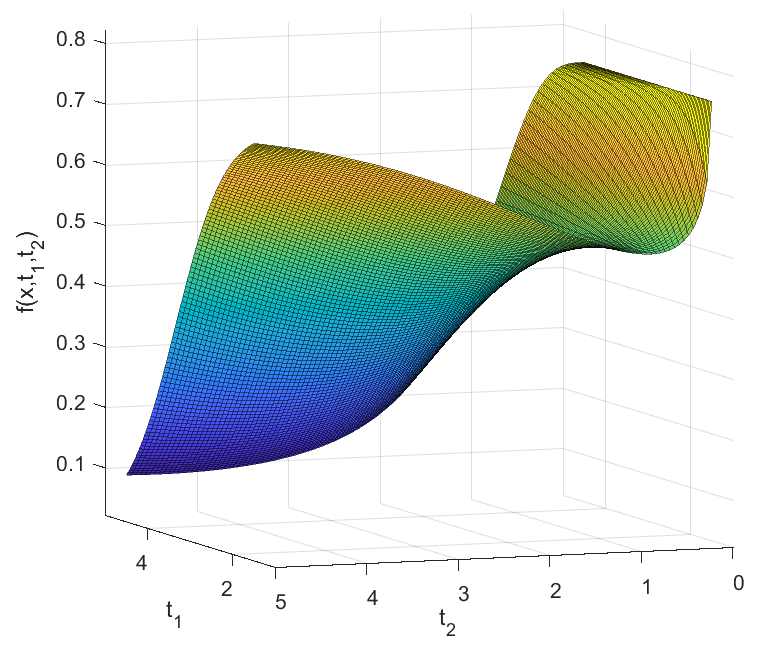
\includegraphics[scale=0.85]{FIG_obj_fn}
\captionsetup{width=.85\linewidth}
\caption{Example computer model output over the support of the calibration parameter $t_c$ and the design parameter $t_d$.}
\label{fig:example_output}
\end{figure}
%
We arbitrarily set $\theta_c=2$ to be the ``true'' value of $t_c$.
%
For any value of $x$ and $t_c$, the optimal (minimizing) value of $t_d$ is $(4/3)(t_c-1)$, so we have $\theta_d=4/3.$
%
Figure \ref{fig:true_vals} shows the locations of the true and optimal values (respectively) of $\theta_c$ and $\theta_d$.
%
\begin{figure}
\centering
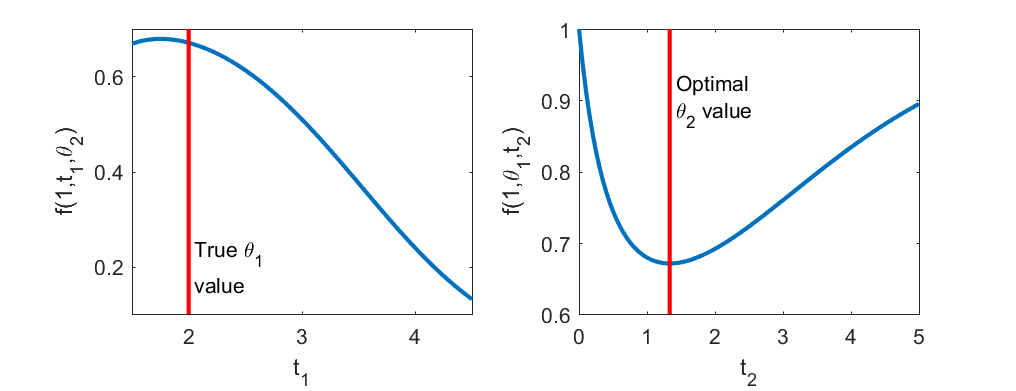
\includegraphics[scale=0.85]{FIG_true_optimal_theta1_theta2}
 	\captionsetup{width=.85\linewidth}
\caption{The lefthand plot shows the computer model output at $x=1$ and optimal $\theta_d$ for each value of the calibration parameter $t_c$. The righthand plot show the model output at $x=1,t_c=\theta_c$ for each value of the design parameter $t_d$.}
\label{fig:true_vals}
\end{figure}
%
There it is clear that the true value of $\theta_c$ is far from optimal -- if this value were within our control, its optimal value would be at the upper end of its support, at 4.5.
%
Thus $\eta$ showcases the ability of DCTO to perform simultaneously both calibration and design in the case when our ``truth-seeking'' goals and our design goals are in tension.
%

%
\subsection{Results}
% 
We used DCTO on four versions of the problem.
%
First, we assumed that $\eta$ is free from discrepancy -- i.e. that $\eta(x,\theta_c,t_d)$ is an unbiased estimator of the ``true'' system $f(x,t_d)$.
%
The other three versions each assume that $\eta$ suffers from some form of discrepancy.
%
Let $f_1,f_2,f_3$ denote the ``true'' systems in these three cases.
%
We set 
\begin{align*}
f_1(x,t_d) &= \eta(x,\theta_c,t_d) \left(1-a(x-.5)(x-1)/x) \right) \\
f_2(x,t_d)&= \eta(x,\theta_c,t_d) - a(x-.5)(x-1)\left(t_d-\frac43\right)^2 + b\\
f_3(x,t_d)&=\eta(x,\theta_c,t_d) + axt_d+b
\end{align*}
%
Where $a,b$ are constants which determine how severe the discrepancy is in each case.
%
The function $f_1$ has a multiplicative discrepancy dependent only on $x$. 
%
This discrepancy does not affect the optimal value of $t_d$.  
%
The discrepancy of $f_2$ is additive, and is dependent upon both $x$ and $\theta_c$. 
%
Though this discrepancy can affect the optimal value of $t_d$, in the case that $\theta_c=2$ (which is what we assume to be the truth) it does not.
%
Thus under $f_1$ and $f_2$, it remains the case that the optimal value of $t_d$ is $\theta_d=4/3$. 
%
By contrast, $f_3$ has an additive discrepancy which does affect the optimal setting for $t_d$. 
%
For $f_3$, optimal $t_d$ is dependent upon both the true value of $\theta_c$ and upon the value of $a$. 
%
For example, for $\theta_c=2$ and $a=0.055$, the optimal $t_d$ is $\theta_d\approx1$.
%
Figure \ref{fig:discrepancies} shows the discrepancies for two different versions (corresponding to different settings of $(a,b)$) of each $f_i$.
%
\begin{figure}
\centering
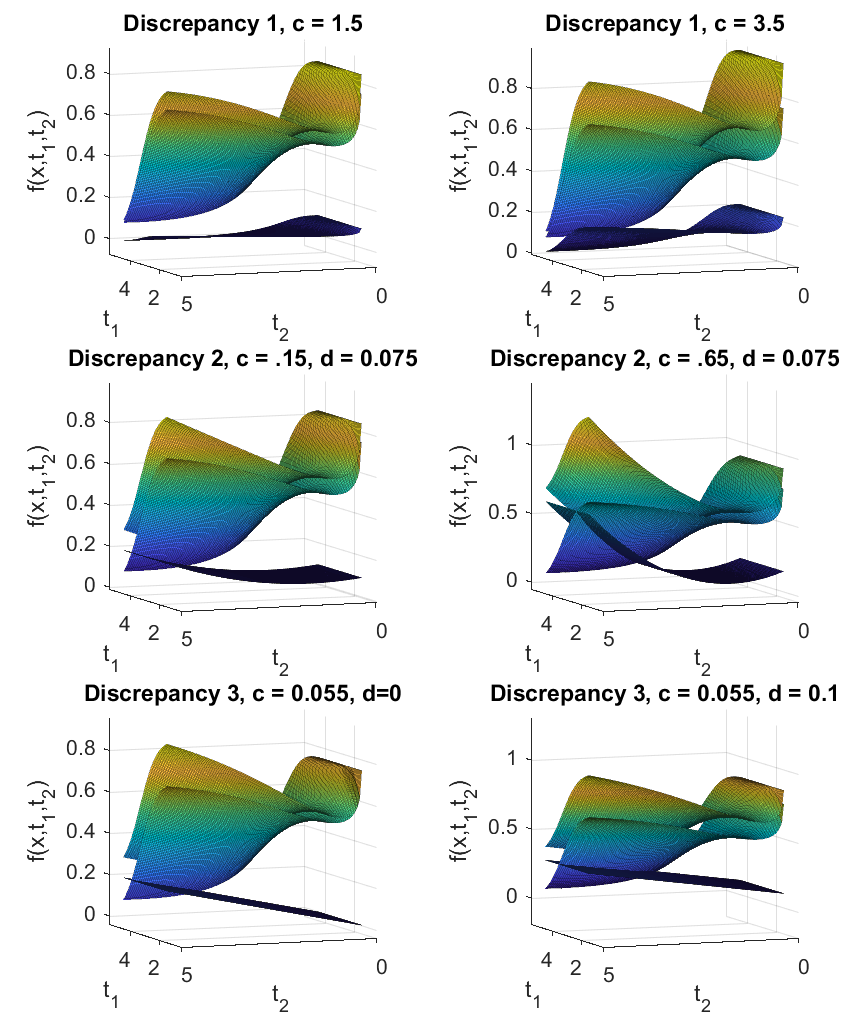
\includegraphics[scale=0.85]{FIG_six_discrepancies}
\captionsetup{width=.85\linewidth}
\caption{The $i^{\text{th}}$ row shows $f_i$ (the objective function with discrepancy), $\eta$ (the computer model), and the discrepancy $f_i-\eta$, all at $x=0.75$. In each row, a less aggressive version of the discrepancy appears on the left, and a more aggressive on the right. In each plot, the topmost surface is $f_i$, the middle surface is $\eta$, and the bottom surface is the discrepancy $f_i-\eta$.}
\label{fig:discrepancies}
\end{figure}
%

%
We applied DCTO to each of seven cases: the non-discrepancy case, and the two different versions of each $f_i$ shown in Figure \ref{fig:discrepancies}.
%
We found that in these cases, no appreciable difference resulted from the decision of whether or not to use an emulator (where the emulator was trained on a latin hypercube design of 250 points on the space of model inputs).
%
Therefore, the results reported here do not employ an emulator.
%
In each case, we gathered 50 ``observations'' of $f_i$ on a latin hypercube design over the supports of $x$ and $\theta_d$, setting $\theta_c$ equal to its ``true'' value of 2.
%
After standardizing the response to have mean 0 and standard deviation 1, we added i.i.d.\ N(0,0.05) noise to the response.
%
We then carried out DCTO using Metropolis-Hastings-within-Gibbs MCMC, drawing 8000 samples each of $t_c,t_d,\boldsymbol\rho_{\delta},\lambda_{\delta},\sigma^2_d$, where $\boldsymbol\phi_\delta = (\boldsymbol\rho_\delta^T,\lambda_\delta)^T$.
%
We modularized the analysis by drawing each of $\boldsymbol\theta_c,\boldsymbol\rho_\delta,\lambda_\delta$ using the likelihood based only on $\mathbf y_r$ rather than on $\mathbf y$.
%

%
In order to evaluate the success of the calibration component of DCTO, we also carried out a two-step procedure of using traditional KOH calibration of $\theta_c$, followed by a second step using CTO to obtain a distribution of $\theta_d$. 
%In the first step of this KOH+CTO procedure, we re-running the procedure with $\mathbf{x_d},\mathbf{y_d}$ as empty (null) vectors, followed by CTO calibration of $\theta_2$ using the 
%
The first step is essentially DCTO with $\mathbf{x_d},\mathbf{y_d}$ as empty (null) vectors, and the second step uses the distributions obtained in the first step to estimate $\theta_d$.
%
Thus, the comparison between DCTO and KOH+CTO shows the difference between DCTO and performing CTO on a system which has been calibrated using traditional methods.
%
%In doing so, we would hope to find that DCTO and KOH give similar posterior distributions for $\theta_1$, and that DCTO gives a posterior distribution of $\theta_2$ peaked at its optimal value while KOH gives a posterior distribution that approximates the (uniform) prior.
%
Figure \ref{fig:no_discrep_results} shows the results of DCTO and KOH+CTO for $f_0$, the case of no discrepancy.
%
\begin{figure}
\centering
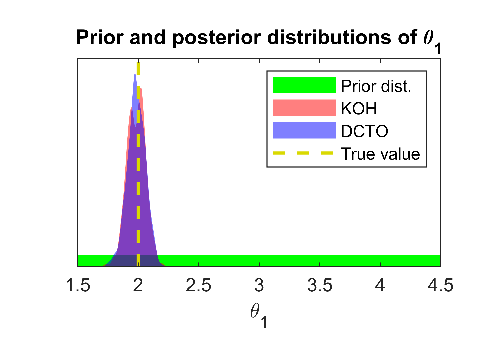
\includegraphics[scale=0.85]{FIG_dual_calib_post_theta1-d0}
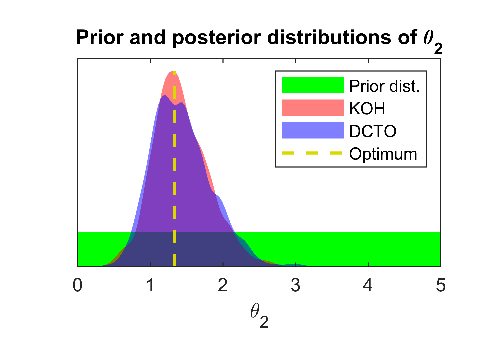
\includegraphics[scale=0.85]{FIG_dual_calib_post_theta2-d0}
\captionsetup{width=.85\linewidth}
\caption{Prior and posterior distributions of the calibration parameter $\theta_1$ and design parameter $\theta_2$, along with their true/optimal values, for DCTO and KOH+CTO carried out when there is no discrepancy between the true system and the computer model.}
\label{fig:no_discrep_results}
\end{figure}
%
The two methods deliver comparable results, illustrating that combining KOH calibration and CTO design into DCTO does not undermine the performance of either task.
%
Strong Bayesian learning has occurred for both parameters, in that the posterior distributions of $\theta_1,\theta_2$ are peaked around their true and optimal values, respectively.
%
KOH gives a similar posterior for $\theta_1$, showing that the expansion of DCTO to undertake design has not interfered with its calibration performance.
%
The skewness apparent in the posterior distributions of $\theta_2$ occur in all of the results gathered here, and is likely due to the shape of the objective function $f$, which increases sharply for $t_2<\theta_2$ and increases much more gently for $t_2>\theta_2$.
%

%
We performed each procedure 30 times on each of the seven different discrepancy situations (no discrepancy, and a large and small version of each of three discrepancies).
%
The results are summarized in Table \ref{table:vars_and_rmses}.
%
\begin{table}[]
	\centering
	\begin{tabular}{l|cc|cc}
		&\multicolumn{2}{c|}{Posterior $\theta_c$ var.}&
		\multicolumn{2}{c}{Posterior $\theta_d$ var.} \\ \hline
		Discrepancy    & DCTO   & KOH+CTO & DCTO    & KOH+CTO   \\ \hline
		0              & 0.00633 & 0.00619 & 0.145 & 0.129\\ \hline
		1, small       & 0.0140 & 0.0137 & 0.149 & 0.129\\ \hline
		1, large       & 0.0141 & 0.0140 & 0.149 & 0.131\\ \hline
		2, small       & 0.0143 & 0.0141 & 0.135 & 0.116\\ \hline
		2, large       & 0.0609 & 0.0608 & 0.0804 & 0.0731\\ \hline
		3, small       & 0.0134 & 0.0135 & 0.0882 & 0.0743\\ \hline
		3, large       & 0.0143 & 0.0142 & 0.0945 & 0.0814\\ \hline
	\end{tabular}\\
	\vspace{.25in}
	\begin{tabular}{l|cc|cc}
		&\multicolumn{2}{c|}{$\widehat\theta_c$ RMSE}&
		\multicolumn{2}{c}{$\widehat\theta_d$ RMSE} \\ \hline
		Discrepancy    & DCTO   & KOH+CTO & DCTO    & KOH+CTO   \\ \hline
		0              & 0.0790 & 0.0795 & 0.120 & 0.121\\ \hline
		1, small       & 0.0955 & 0.0956 & 0.149 & 0.144\\ \hline
		1, large       & 0.137 & 0.139 & 0.209 & 0.209\\ \hline
		2, small       & 0.109 & 0.106 & 0.130 & 0.127\\ \hline
		2, large       & 0.158 & 0.155 & 0.123 & 0.121\\ \hline
		3, small       & 0.294 & 0.292 & 0.0919 & 0.0919\\ \hline
		3, large       & 0.279 & 0.281 & 0.0995 & 0.0990\\ \hline
	\end{tabular}
	\caption{Posterior variance and root mean square error (RMSE) for the calibration variable $\theta_1$ and the design variable $\theta_2$ under both DCTO and KOH+CTO. The estimator $\widehat{\theta_i}$ is the posterior mean of $t_i$.} 
	\label{table:vars_and_rmses}
\end{table}
%
The upper table gives the sample mean, over the thirty runs, of the marginal posterior variance of each of $\theta_c$ and $\theta_d$.
%
The two procedures generate extremely similar outcomes with respect to $\theta_c$.
%
However, the posterior variance for $\theta_d$ under DCTO is slightly higher than that under CTO in each of the seven cases considered.
%
This is due to the fact that DCTO includes remaining uncertainty about the values of the hyperparameters of the discrepancy GP $\delta()$.
%
By contrast, CTO after KOH uses point estimates of those hyperparameters and thus achieves narrower posterior distributions due to excluding this source of uncertainty.
%
The lower table gives the root mean square errors (RMSEs) for the posterior means of $\theta_c$ and $\theta_d$, using their true value of 2 for $\theta_c$ and optimal value $4/3$ for $theta_d$ in discrepancy cases $0-2$ and $1$ for discrepancy 3.
%
Again we see very similar outcomes in the two procedures for both parameters.
%
In all cases but one, DCTO has slightly higher RMSE for $\theta_d$ than does CTO.
%
This is to be expected given the above-mentioned wider posterior distributions of $\theta_d$ under DCTO.
%

%
\section{Dependence of $\theta_c$ on $\theta_d$}\label{sec:as}
%
In many cases of computer model calibration, it is known or suspected that the value of one or more calibration parameters are functionally dependent upon the values of other model inputs \citep{Atamturktur2015,Atamturktur2017,Ezzat2018}.
%
If one is interested to understand the functional form of the calibration parameter, then state-aware methods can be used to arrive at such an estimate \citep{Atamturktur2015,Atamturktur2017}.
%
However, in a case of simultaneous calibration and design in which the calibration parameter is functionally dependent upon the design settings, one might be interested only to know the value of the calibration parameter in the optimal design region.
%
In this case, the machinery of state-aware calibration is not needed, and effort is better spent focusing on estimating the fixed calibration parameter value in the region of interest.
%
In such a case, it is preferable that one's calibration be founded on observations for which the design settings are in the optimal design region.
%
This will allow one to calibrate the model using observations taken from the region of interest, so that the calibration takes on values from that region.
%

%
Recall that when observations may be made adaptively, other RSM approaches such as EGO \citep{Jones1998,Brochu2010} or SUR \citep{Geman1996,Villemonteix2009,Chevalier2014,Picheny2015,MiguelHernandez-Lobato2016,Picheny2019,Binois2019} may be more efficient than CTO for estimating optimal design settings, though CTO offers more interpretable and model-driven uncertainty quantification.
%
However, RSM approaches in general do not include tools to accommodate the case in which a model stands in need of calibration as well as optimization.
%
DCTO provides such a framework for combined calibration and design.
%
Therefore we now consider under the lens of DCTO the case in which the design settings of the observations of the true system may be chosen adaptively.
%

%
An obvious approach when both calibration and design are undertaken and the calibration parameter is suspected to be functionally dependent on the design settings is to perform the design optimization first, and then the calibration.
%
In this way, one would gather observations in service of finding the optimal design settings, and then use these observations to learn the value of the calibration parameter in the associated optimal design region.
%
For this purpose, any optimization method could be used to select the design settings for the observations.
%
If a limited budget of observations is available and quantification of remaining uncertainty surrounding the true and optimal values (respectively) of the calibration parameter and design settings is desired, then RSMs are a good choice.
%
In such a situation, CTO retains its advantage of interpretable and model-driven uncertainty quantification, and adds another advantage: namely, that DCTO constitutes a method for combining both the observations of the true system and the existing uncalibrated computer model to select new evaluation points.
%

%
The use of DCTO with adaptive sampling is potentially of greatest use when it is known or suspected that the calibration parameter is a function $\theta_c(t_d)$ of the design setting $t_d$, and particularly when interest focuses on learning the optimal design setting $\theta_d$ and the corresponding value $\theta_c(\theta_d)$ of the calibration parameter.
%
To implement DCTO with adaptive sampling in such a case, we perform DCTO beginning with an empty vector of true observations $y_r$.
%
During the burn-in period, every (e.g.) 100 iterations of the MCMC, we sample draw a sample $\widehat\theta_d$ from the posterior distribution of the design settings $t_d$, as a means of estimating the optimal design settings $\theta_d$.
%
We then perform a new observation of the system at $(\mathbf x_i,\widehat\theta_d)$ where $i\in\{1,\cdots,m\}$ and $m$ is the total budget of observations to be made.
%
The non-design input settings $\mathbf x_i$ can be chosen to maximize distance from previous observations, or these locations can be predetermined according to a space-filling design over the domain $\mathcal X$ of non-design inputs.
%
This process is continued until the total budget of observations is reached, after which burn-in continues until the MCMC chains converge for all parameters of interest.
%
The result is that observations are concentrated around the design settings of interest, so that the unknown calibration parameter values in those observations are concentrated around the value $\theta_c(\theta_d)$.
%

%
To demonstrate the use of DCTO with adaptive sampling in a case of functional dependence of the calibration parameter on design settings, we use the same objective function and discrepancy cases as described in Section \ref{sec:example}.
%
This time, instead of setting $\theta_c = 2$, we set 
\[\theta_c(t)= 2.25 - .75 \frac{ \exp\left(40\left(\frac{t-1.5}{.75}-.5\right)\right)} {1 + \exp\left( 40\left(\frac{t-1.5}{.75}-.5\right) \right)}.\]
%
The resulting optimal design settings and calibration parameter value at the optimum vary in the discrepancy cases, though $\theta_c(\theta_d)$ is near 2.16 in each case.
%
Representative results from performing DCTO with adaptive sampling in each discrepancy case appear in Figure \ref{fig:sdoe_vs_pdoe}, along with results from applying DCTO non-adaptively (using a space-filling set of observations).
%
A summary of the results of thirty applications of DCTO both with and without adaptive sampling, for each of the discrepancy cases, appears in Table \ref{table:vars_and_rmses}
%
\begin{figure}
	\centering
	\begin{tabular}{c c c}
	$g_0$ &
	\raisebox{-.5\height}{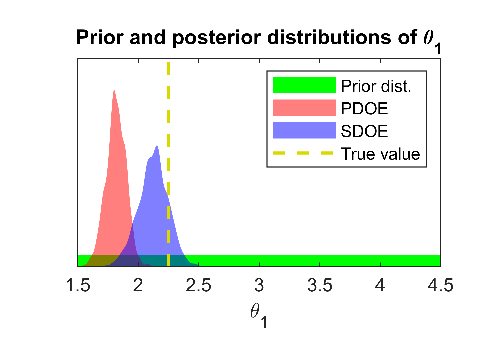
\includegraphics[scale=0.85]{FIG_dual_calib_SDOE_comp_theta1-d0}} &
	\raisebox{-.5\height}{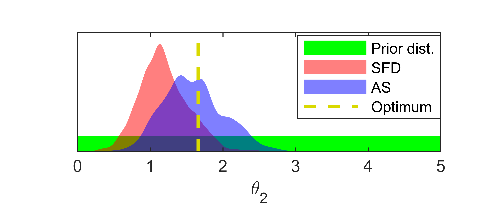
\includegraphics[scale=0.85]{FIG_dual_calib_SDOE_comp_theta2-d0}}\\
	$g_1$, small & 
	\raisebox{-.5\height}{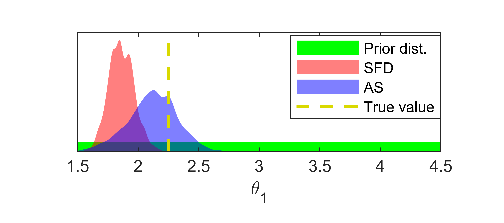
\includegraphics[scale=0.85]{FIG_dual_calib_SDOE_comp_theta1-d1}} &
	\raisebox{-.5\height}{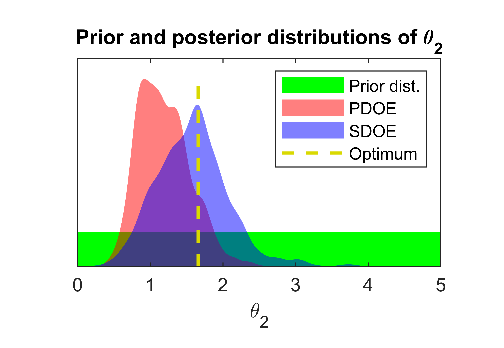
\includegraphics[scale=0.85]{FIG_dual_calib_SDOE_comp_theta2-d1}}\\
	$g_1$, large & 
	\raisebox{-.5\height}{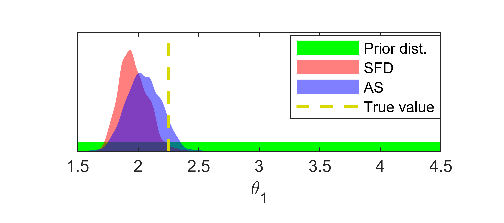
\includegraphics[scale=0.85]{FIG_dual_calib_SDOE_comp_theta1-d2}} &
	\raisebox{-.5\height}{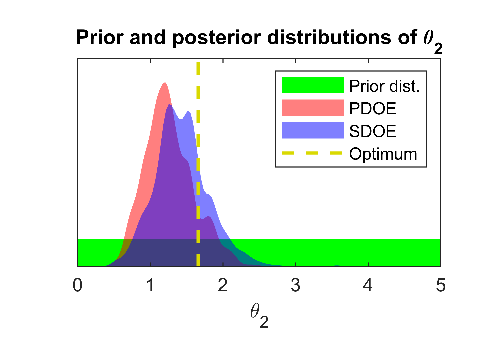
\includegraphics[scale=0.85]{FIG_dual_calib_SDOE_comp_theta2-d2}}\\
	$g_2$, small &
	\raisebox{-.5\height}{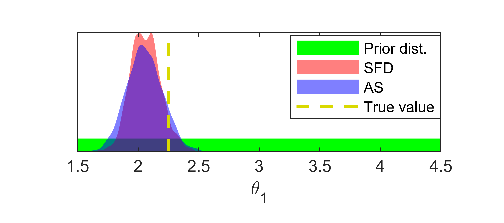
\includegraphics[scale=0.85]{FIG_dual_calib_SDOE_comp_theta1-d3}} &
	\raisebox{-.5\height}{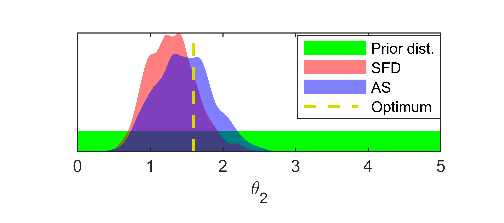
\includegraphics[scale=0.85]{FIG_dual_calib_SDOE_comp_theta2-d3}}\\
	$g_2$, large &
	\raisebox{-.5\height}{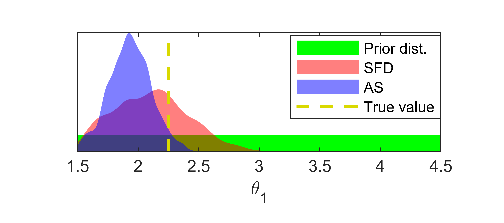
\includegraphics[scale=0.85]{FIG_dual_calib_SDOE_comp_theta1-d4}} &
	\raisebox{-.5\height}{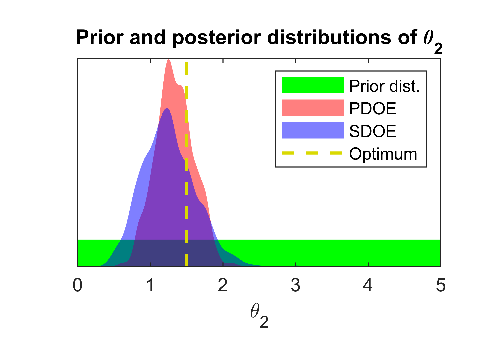
\includegraphics[scale=0.85]{FIG_dual_calib_SDOE_comp_theta2-d4}}\\
	$g_3$, small &
	\raisebox{-.5\height}{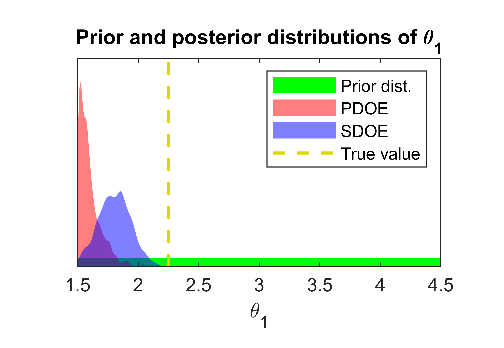
\includegraphics[scale=0.85]{FIG_dual_calib_SDOE_comp_theta1-d5}} &
	\raisebox{-.5\height}{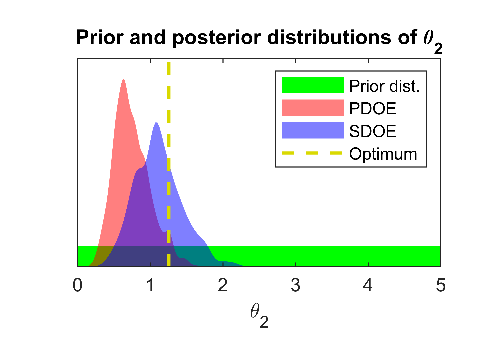
\includegraphics[scale=0.85]{FIG_dual_calib_SDOE_comp_theta2-d5}}\\
	$g_3$, large &
	\raisebox{-.5\height}{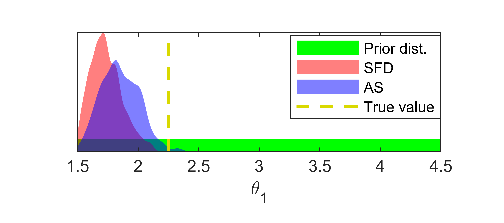
\includegraphics[scale=0.85]{FIG_dual_calib_SDOE_comp_theta1-d6}} &
	\raisebox{-.5\height}{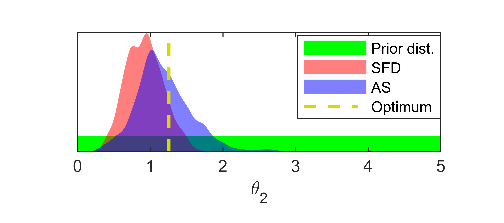
\includegraphics[scale=0.85]{FIG_dual_calib_SDOE_comp_theta2-d6}}
	\end{tabular}
	\captionsetup{width=.85\linewidth}
	\caption{Prior and posterior distributions of the calibration parameter $\theta_1$ and design parameter $\theta_2$, along with their true/optimal values, for DCTO with adaptive sampling (AS) and with predetermined space-filling design (SFD).}
	\label{fig:sdoe_vs_pdoe}
\end{figure}
%
\begin{table}[]
	\centering
	\begin{tabular}{l|cc|cc}
		&\multicolumn{2}{c|}{$\widehat\theta_c$ RMSE}&
		\multicolumn{2}{c}{$\widehat\theta_d$ RMSE} \\ \hline
		Discrepancy    & AS   & SFD & AS    & SFD   \\ \hline
		0              & 0.188 & 0.433 & 0.163 & 0.479\\ \hline
		1, small       & 0.233 & 0.32 & 0.243 & 0.414\\ \hline
		1, large       & 0.188 & 0.247 & 0.213 & 0.393\\ \hline
		2, small       & 0.221 & 0.263 & 0.187 & 0.348\\ \hline
		2, large       & 0.228 & 0.16 & 0.183 & 0.206\\ \hline
		3, small       & 0.452 & 0.506 & 0.182 & 0.329\\ \hline
		3, large       & 0.448 & 0.468 & 0.167 & 0.292\\ \hline
	\end{tabular}
	\caption{Posterior root mean square error (RMSE) for the calibration variable $\theta_1$ and the design variable $\theta_2$, for DCTO with adaptive sampling (AS) and a predetermined space-filling design (SFD). The estimator $\widehat{\theta_i}$ is the posterior mean of $t_i$.} 
	\label{table:vars_and_rmses}
\end{table}
%

%
The results show superior performance for the adaptive sampling DCTO over DCTO using a space-filling design.
%
The adaptive DCTO posterior means have lower RMSEs in all cases for $\theta_d$, and in all cases except one for $\theta_c$.
%
This demonstrates a useful robustness of adaptive DCTO to model misspecification, specifically in the case that the model treats as constant a calibration parameter that is more properly understood as functionally dependent upon other model inputs.
%
By using the CTO-driven estimate $\widehat\theta_d$ to sample from the region of interest, DCTO learns from observations such that $\theta_c(\widehat\theta_d)$ is near to the value $\theta_c(\theta_d)$.
%
This promotes better calibration with respect to the region of interest, and thereby better estimation of the optimal design settings.
%
By relying on DCTO rather than on performing KOH using samples gathered using heuristic optimization methods, or other RSM approaches, we achieve these estimates with quantification of all relevant model-driven uncertainty with respect to the values of $\theta_c$ and $\theta_d$.
%

\bigskip

%\begin{center}
%{\large\bf SUPPLEMENTARY MATERIAL}
%\end{center}
%
%\begin{description}
%
%\item[Title:] Brief description. (file type)
%
%\item[R-package for  MYNEW routine:] R-package �MYNEW� containing code to perform the diagnostic methods described in the article. The package also contains all datasets used as examples in the article. (GNU zipped tar file)
%%
%\item[HIV data set:] Data set used in the illustration of MYNEW method in Section~ 3.2. (.txt file)
%
%\end{description}

\bibliographystyle{Chicago}

\bibliography{lit_review}
\end{document}

\begin{figure}
\begin{center}
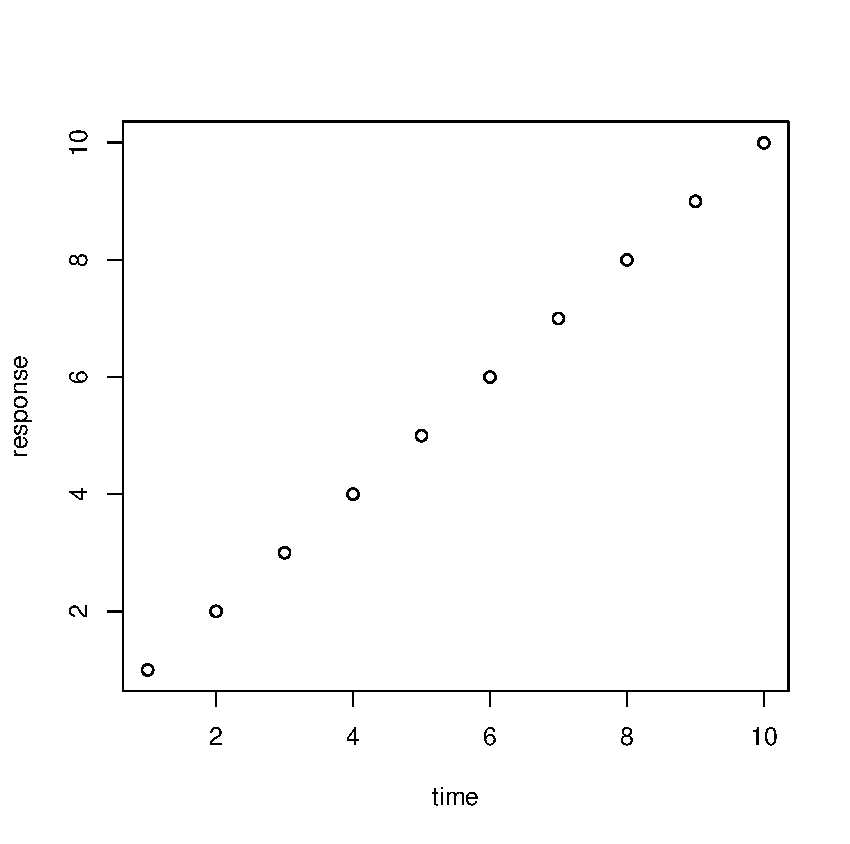
\includegraphics[width=3in]{fig1.pdf}
\end{center}
\caption{Consistency comparison in fitting surrogate model in the tidal
power example. \label{fig:first}}
\end{figure}

\begin{table}
\caption{D-optimality values for design $X$ under five different scenarios.  \label{tab:tabone}}
\begin{center}
\begin{tabular}{rrrrr}
one & two & three & four & five\\\hline
1.23 & 3.45 & 5.00 & 1.21 & 3.41 \\
1.23 & 3.45 & 5.00 & 1.21 & 3.42 \\
1.23 & 3.45 & 5.00 & 1.21 & 3.43 \\
\end{tabular}
\end{center}
\end{table}

\begin{itemize}
\item Note that figures and tables (such as Figure~\ref{fig:first} and
Table~\ref{tab:tabone}) should appear in the paper, not at the end or
in separate files.
\item In the latex source, near the top of the file the command
\verb+\newcommand{\blind}{1}+ can be used to hide the authors and
acknowledgements, producing the required blinded version.
\item Remember that in the blind version, you should not identify authors
indirectly in the text.  That is, don't say ``In Smith et. al.  (2009) we
showed that ...''.  Instead, say ``Smith et. al. (2009) showed that ...''.
\item These points are only intended to remind you of some requirements.
Please refer to the instructions for authors
at \url{http://www.tandfonline.com/action/authorSubmission?journalCode=utch20&page=instructions#.UieFdDafgx0}
\item If you have Supplementary Material (eg software, data, technical
proofs), identify them in the section below.  In early stages of the
submission process, you may be unsure what to include as supplementary
material.  Don't worry---this is something that can be worked out at later stages.
\end{itemize}
